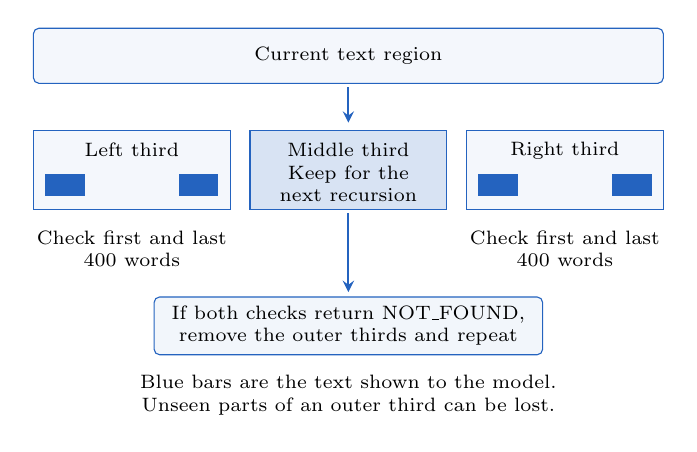
\begin{tikzpicture}[x=1cm,y=1cm,font=\scriptsize,>=stealth]
\definecolor{rbrblue}{RGB}{36,99,191}
\draw[draw=rbrblue,fill=rbrblue!5,rounded corners=2pt] (0,0) rectangle (8,0.7);
\node at (4,0.35) {Current text region};
\draw[->,rbrblue,thick] (4,-0.05) -- (4,-0.5);
\draw[draw=rbrblue,fill=rbrblue!5] (0,-1.6) rectangle (2.5,-0.6);
\draw[draw=rbrblue,fill=rbrblue!18] (2.75,-1.6) rectangle (5.25,-0.6);
\draw[draw=rbrblue,fill=rbrblue!5] (5.5,-1.6) rectangle (8,-0.6);
\node at (1.25,-0.85) {Left third};
\node at (4,-0.85) {Middle third};
\node at (6.75,-0.85) {Right third};
\foreach \position in {0.15,1.85,5.65,7.35} {\fill[rbrblue] (\position,-1.43) rectangle +(0.5,0.28);}
\node[align=center] at (4,-1.28) {Keep for the\\next recursion};
\node[align=center] at (1.25,-2.1) {Check first and last\\400 words};
\node[align=center] at (6.75,-2.1) {Check first and last\\400 words};
\draw[->,rbrblue,thick] (4,-1.65) -- (4,-2.65);
\node[draw=rbrblue,rounded corners=2pt,fill=rbrblue!6,align=center,text width=4.7cm] at (4,-3.08) {If both checks return NOT\_FOUND,\\remove the outer thirds and repeat};
\node[align=center,text width=7.6cm] at (4,-3.96) {Blue bars are the text shown to the model.\\Unseen parts of an outer third can be lost.};
\end{tikzpicture}
